\documentclass[prb,twocolumn,showpacs,preprintnumbers,amsmath,amssymb, superscriptaddress]{revtex4-2}

%\usepackage[magyar]{babel}
%\usepackage[makeroom]{cancel}
\usepackage{amsmath}    % need for subequations
\usepackage{amssymb}
\usepackage{graphicx}   % need for figures
\usepackage{verbatim}   % useful for program listings
\usepackage{color}      % use if color is used in text
%\usepackage{subfigure}  % use for side-by-side figures
\usepackage{hyperref}   % use for hypertext links, including those to external documents and URLs
%\usepackage{blindtext}
\usepackage[normalem]{ulem}
%\usepackage{xpatch}
\usepackage{natbib}
\usepackage{fixmath}
\usepackage{enumitem}
\usepackage{dsfont}
\usepackage{subcaption}

\def \brc #1{\left\lbrace #1 \right\rbrace}
\def \loc {\mathrm{loc}}


\hypersetup{colorlinks,linkcolor=blue,urlcolor=blue,citecolor=blue}
\newcommand{\uv}[1]{\ensuremath{\mathbf{\hat{#1}}}} % for unit vector
\newcommand{\gv}[1]{\ensuremath{\mbox{\boldmath$ #1 $}}} % 
\newcommand{\rem}[1]{  {\color{red} #1}  }
%\newcommand{\g}[1]{{\bf #1 }} %
\newcommand{\beq}{\begin{equation}}
\newcommand{\eeq}{\end{equation}}
\newcommand{\bea}{\begin{eqnarray}}
\newcommand{\eea}{\end{eqnarray}}
\newcommand{\blabel}{\,b}
\newcommand{\alabel}{\,a}
\newcommand{\Lspace}{{\mathit{\mathbb{L}}}}

\newcommand{\bbGamma}{{\mathpalette\makebbGamma\relax}}
\newcommand{\makebbGamma}[2]{%
  \raisebox{\depth}{\scalebox{1}[-1]{$\mathsurround=0pt#1\mathbb{L}$}}%
}

\newcommand{\e}{\text e}
\newcommand{\zp}{\mathbb Z^+}
\newcommand{\z}{\mathbb Z}
\newcommand{\hint}{H_{\text{int}}}
\newcommand{\re}{\text{Re }}
\newcommand{\hc}{\text{h.c.}}
\newcommand{\cc}{\text{c.c.}}
\newcommand{\w}{\omega}
\newcommand{\be}{\begin{equation}}
\newcommand{\ee}{\end{equation}}
\newcommand{\Nedge}{N_{\rm edge}}



\definecolor{darkgreen}{rgb}{0,0.5,0}
\definecolor{orange}{rgb}{1,0.5,0}
\definecolor{grey}{rgb}{.6,.6,.6}
\newcommand{\rc}[1]{\textcolor{red}{#1}}
%\bibliographystyle{apsrev4-1}
%\newcommand{\jav}[1]{#1}
\newcommand{\scrap}[1]{{\color{orange}{\sout{#1}}}}
\newcommand{\cpm}[1]{{\color{blue}{#1}}}

\newcommand{\dr}{\text d^3r}
\newcommand{\dfi}{\text d\varphi}
\newcommand{\dd}{\text d}
\newcommand{\tr}{\tilde r}
\newcommand{\tn}{\tilde n}
\newcommand{\tz}{\tilde z}
\newcommand{\tc}{\tilde c}
\newcommand{\tS}{\tilde S}


\newcommand{\heff}{H_{\text{eff}}}
\newcommand{\hkin}{H_{\text{kin}}}

\newcommand{\pp}{P^{++}+P^{--}}
\newcommand{\ps}{P^{\text(S)}}
\newcommand{\pa}{P^{\text(A)}}
\newcommand{\psn}{P_{S=0}}
\newcommand{\pse}{P_{S=1}}
\newcommand{\eppn}{E^{+}_{0}}
\newcommand{\eppe}{E^{+}_{1}}
\newcommand{\ese}{E^{\text{(S)}}_{1}}
\newcommand{\esn}{E^{\text{(S)}}_{0}}
\newcommand{\eae}{E^{\text{(A)}}_{1}}
\newcommand{\ean}{E^{\text{(A)}}_{0}}
\newcommand{\kent}{k\in\text{NT}}
\newcommand{\meV}{\,{\rm meV}}
\newcommand{\ie}{{\it i.e. }}
\newcommand{\bra}[1]{\langle #1|}
\newcommand{\ket}[1]{|#1\rangle}
\newcommand{\average}[1]{\langle #1\rangle}

%\newcommand{\scrap}[1]{{\color{red}{\sout{#1}}}}


\newcommand{\bK}{\mathbf K}
\newcommand{\bS}{\mathbf S}
\newcommand{\bk}{\mathbf k}
\newcommand{\bq}{\mathbf q}
\newcommand{\ba}{\mathbf a}
\newcommand{\bC}{\mathbf C}
\newcommand{\bH}{\mathbf H}


\newcommand{\bx}{\mathbf x}
\newcommand{\br}{\mathbf r}
\newcommand{\brp}{{\mathbf r}'}
\newcommand{\bxp}{{\mathbf x}'}


\newcommand{\g}{{\gamma}}
\newcommand{\ds}{\displaystyle}
\newcommand{\1}{{1\hspace*{-0.5ex} \textrm{l} \hspace*{0.5ex}}}

\newcommand{\cL}{{\cal L }}
\newcommand{\fL}{\mathfrak{ L }}
\newcommand{\cH}{{\cal H }}
\newcommand{\fH}{\mathfrak{H }}

\newcommand{\cQ}{{\cal Q}}
\newcommand{\cG}{{\cal G}}
\newcommand{\cg}{{\cal g}}
\newcommand{\cS}{{\cal S}}
\newcommand{\cJ}{{\cal J}}
\newcommand{\cN}{{\cal N}}
\newcommand{\chU}{\hat{\cal U}}
\newcommand{\hU}{{\hat U}}

\newcommand{\ketL}[1]{|#1 )}
\newcommand{\braL}[1]{( #1|}
\newcommand{\averageL}[1]{( #1 )}
\newcommand{\tsigma}{{\tilde \sigma}}

\def\doubleunderline#1{\underline{\underline{#1}}}

\newcommand{\mk}[1]{{\color{blue} #1}}


\newcommand{\tp}[1]{{\color{darkgreen} #1}}

\begin{document}
\title{Theoretical modeling of the collective tunneling of a Wigner necklace}
\author{Dominik  Szombathy}
\affiliation{Department of Theoretical Physics,  Institute of Physics, Budapest University of Technology and Economics,  Budafoki \'ut 8., H-1111 Budapest, Hungary}
\affiliation{MTA-BME Quantum Dynamics and Correlations Research Group, 
Institute of Physics, Budapest University of Technology and Economics,  Budafoki \'ut 8., H-1111 Budapest, Hungary}
\author{Mikl\'os Antal Werner}
\affiliation{Department of Theoretical Physics,  Institute of Physics, Budapest University of Technology and Economics,  Budafoki \'ut 8., H-1111 Budapest, Hungary}
\affiliation{MTA-BME Quantum Dynamics and Correlations Research Group, 
Institute of Physics, Budapest University of Technology and Economics,  Budafoki \'ut 8., H-1111 Budapest, Hungary}
\author{C\u at\u alin Pa\c scu Moca}
\affiliation{Department of Theoretical Physics, Institute of Physics, Budapest University of Technology and Economics, Budafoki \'ut 8., H-1111 Budapest, Hungary}
\affiliation{Department of Physics, University of Oradea,  410087, Oradea, Romania}
\author{Gergely Zar\'and}
\affiliation{Department of Theoretical Physics,  Institute of Physics, Budapest University of Technology and Economics,  Budafoki \'ut 8., H-1111 Budapest, Hungary}
\affiliation{MTA-BME Quantum Dynamics and Correlations Research Group, 
Institute of Physics, Budapest University of Technology and Economics,  Budafoki \'ut 8., H-1111 Budapest, Hungary}
%\affiliation{ BME-MTA Exotic Quantum Phases Group, Institute of Physics, 
%Budapest University of Technology and Economics, H-1111 Budapest, Hungary}
\date{\today}
\begin{abstract}
To be written. 
\end{abstract}
\maketitle

\section{Introduction}
\begin{itemize}
\item Nanotube description
\item Experimental background
\item Wigner Crystal and $r_s$ values in this system
\end{itemize}

\begin{figure}[h!]
    \begin{center}
     \includegraphics[width=0.7\columnwidth]{Experimental_Setup.png}
     \vskip 10pt
     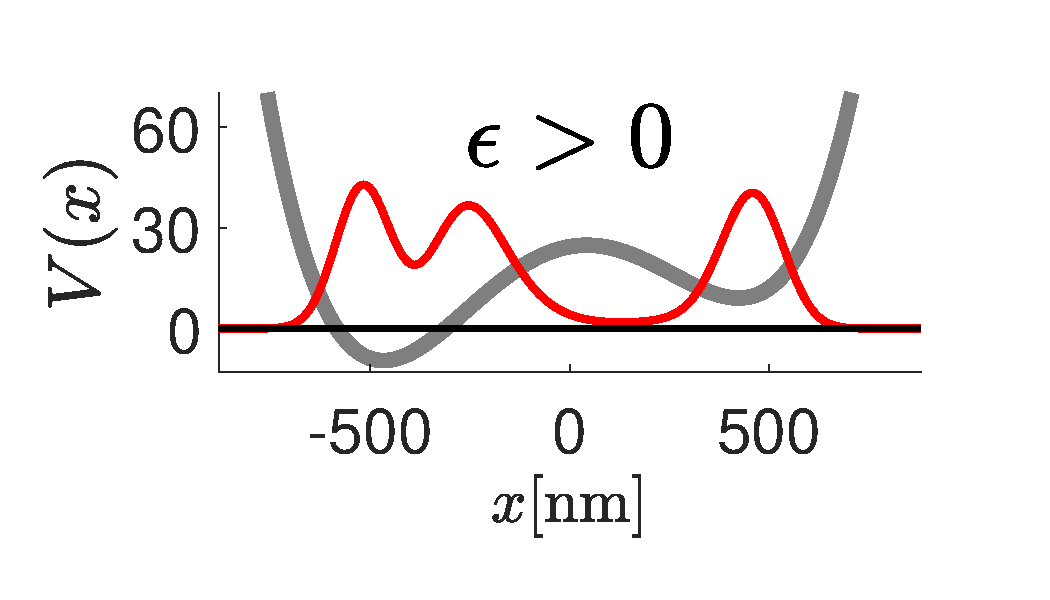
\includegraphics[width=0.49\columnwidth]{Fig_WaveFunction_Potential_NegEps_v1}
     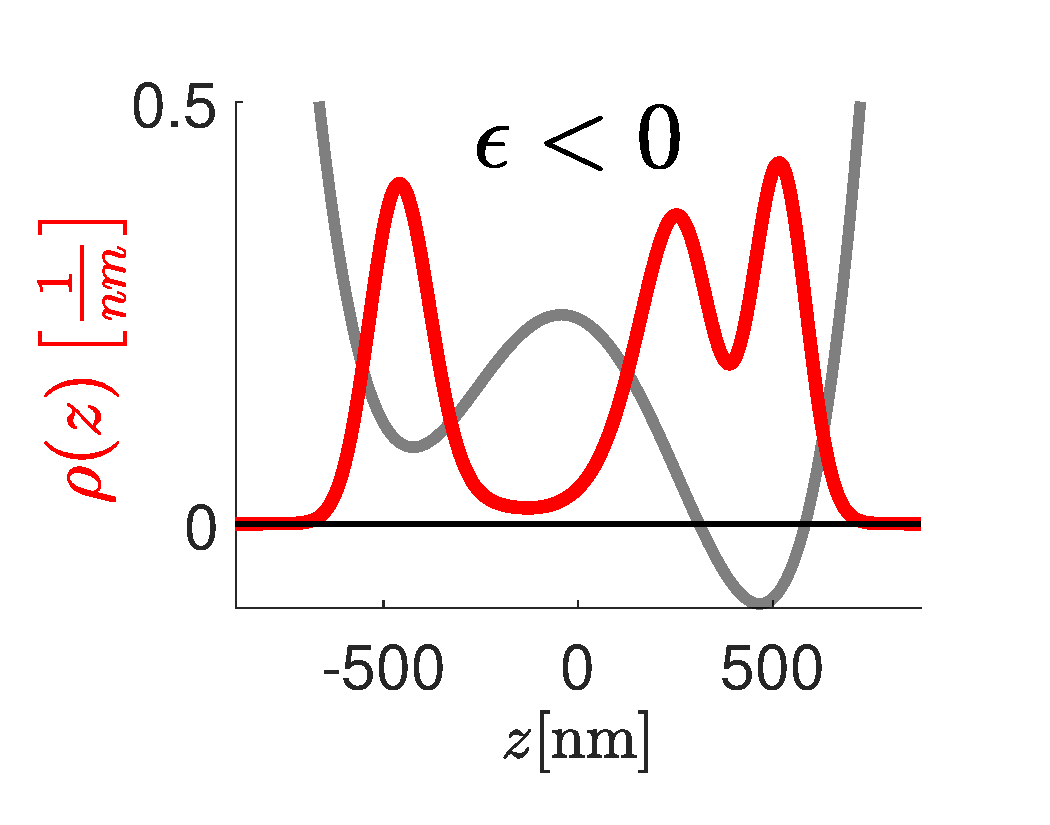
\includegraphics[width=0.49\columnwidth]{Fig_WaveFunction_Potential_PosEps}
    \end{center}
    \caption{Top: Sketch of  the experimental setup used to measure the
	 collective tunneling. The gates  
	 $V_{gi}$ are used to shape the double well potential. 
	 The lefthand side of the nanotube is used as a charge detector. 
	 Bottom: Ground state charge densities  (red) obtained via exact diagonlization  for a the double well potential (grey) with 3 electrons, in the case of finite detuning, $\epsilon$.}
     \label{fig:experimental_setup}
\end{figure}
  
 \begin{figure}[h!]
    \begin{center}
    	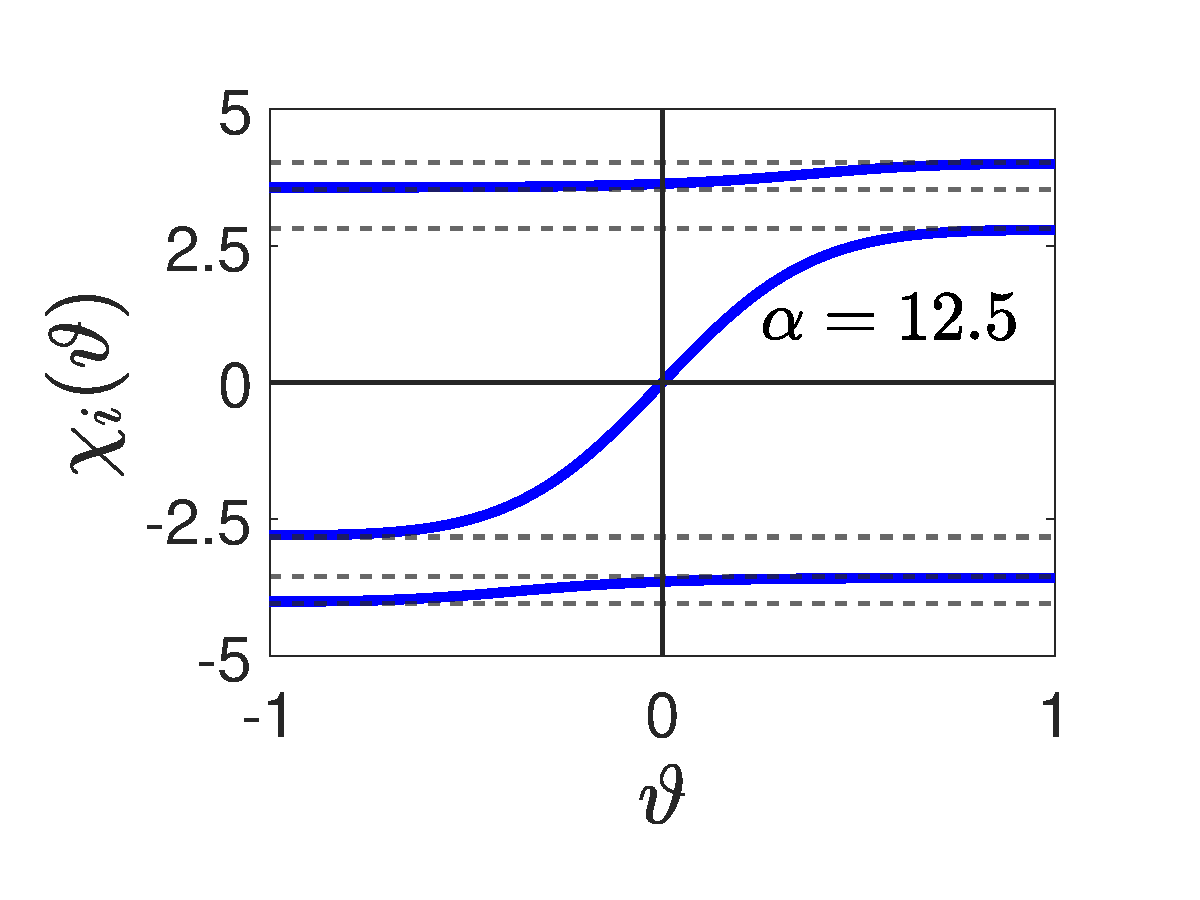
\includegraphics[width=0.49\columnwidth]{Fig_3Particle_Trajectory}
     	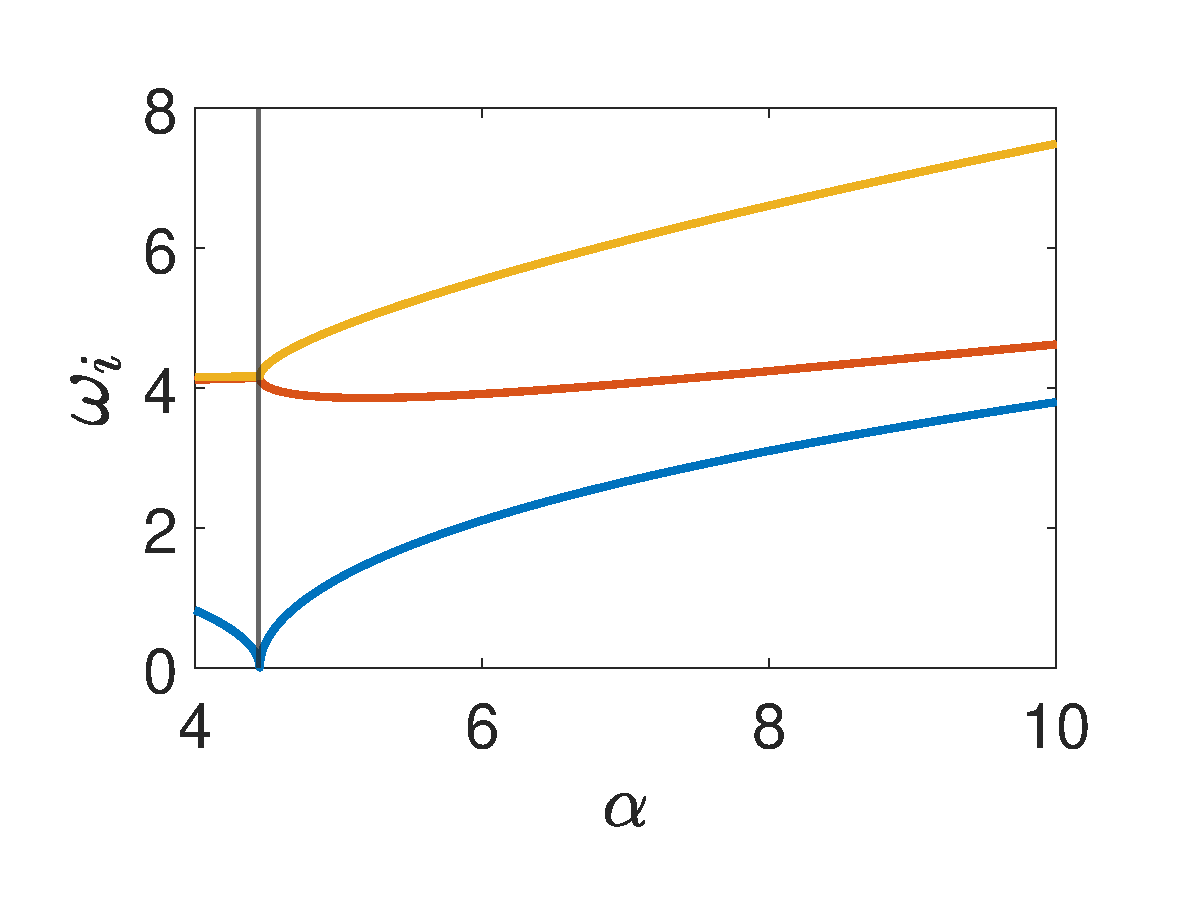
\includegraphics[width=0.49\columnwidth]{SupMatFig_Freqs.pdf}

     \caption{(a) 3 particle imaginary time trajectories (blue) in the natural length scale units for a specific confinement parameter $\alpha = 12.5$. Dashed lines show the classical equilibrium positions or instanton turning points for the 3 particles separately. (b) Harmonic oscillator eigenfrequencies as a function of $\alpha$, in the case of 3 particles. The vertical line marks the beginning of the tunneling regime in the classical calculations $\alpha_{cr}$ value that}
     \label{fig:experimental_setup}
    \end{center}
\end{figure}  

\begin{figure*}[h!]
    \begin{center}
    	\begin{tabular}{cc}
    		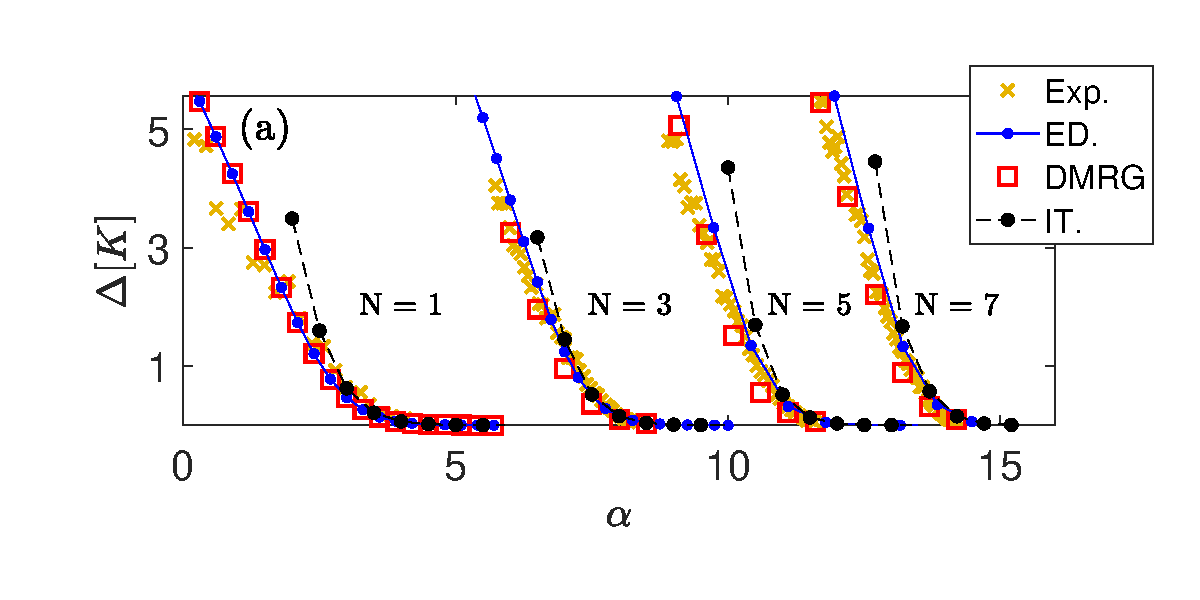
\includegraphics[width=1\columnwidth]{Fig_spectral_gap_exp_fitted_lin}&
    		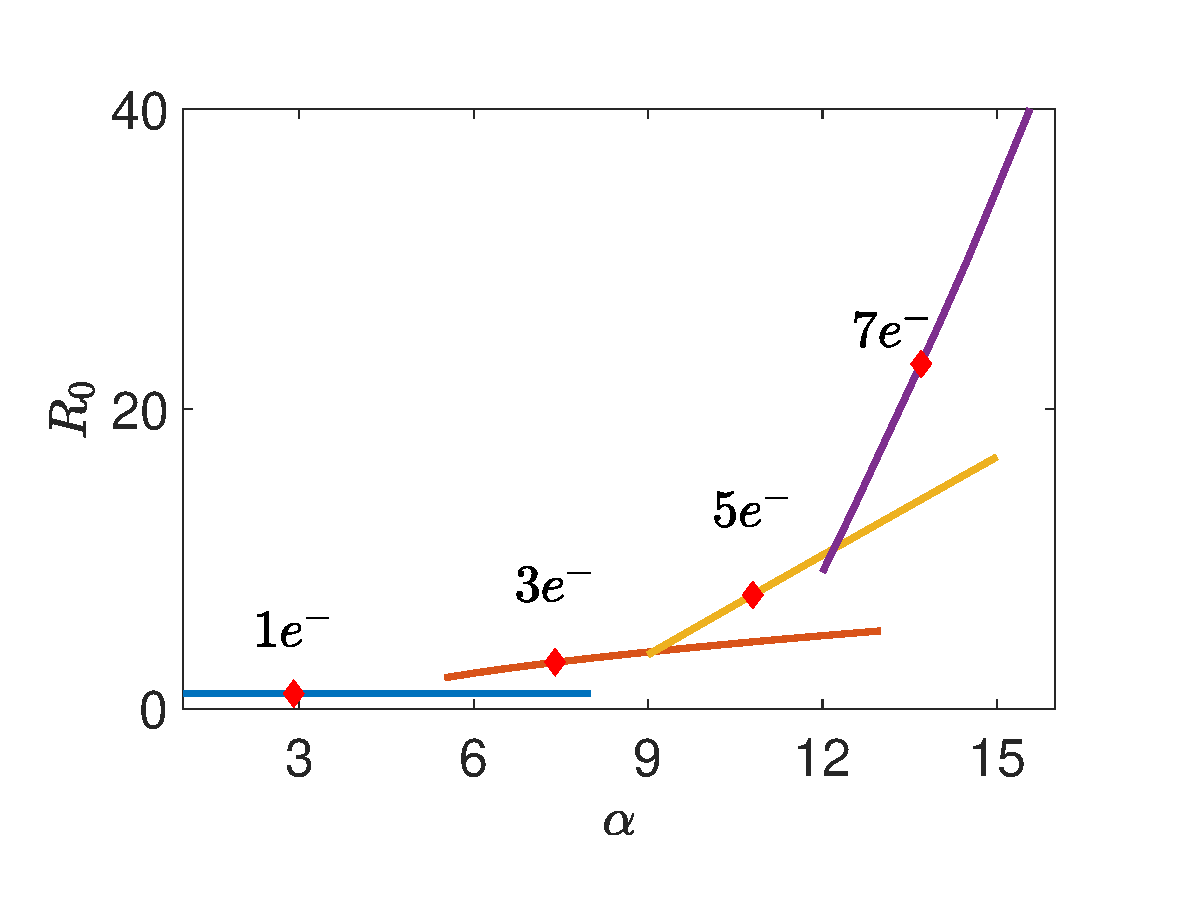
\includegraphics[width=1\columnwidth]{Fig_perpfactors}\\
  			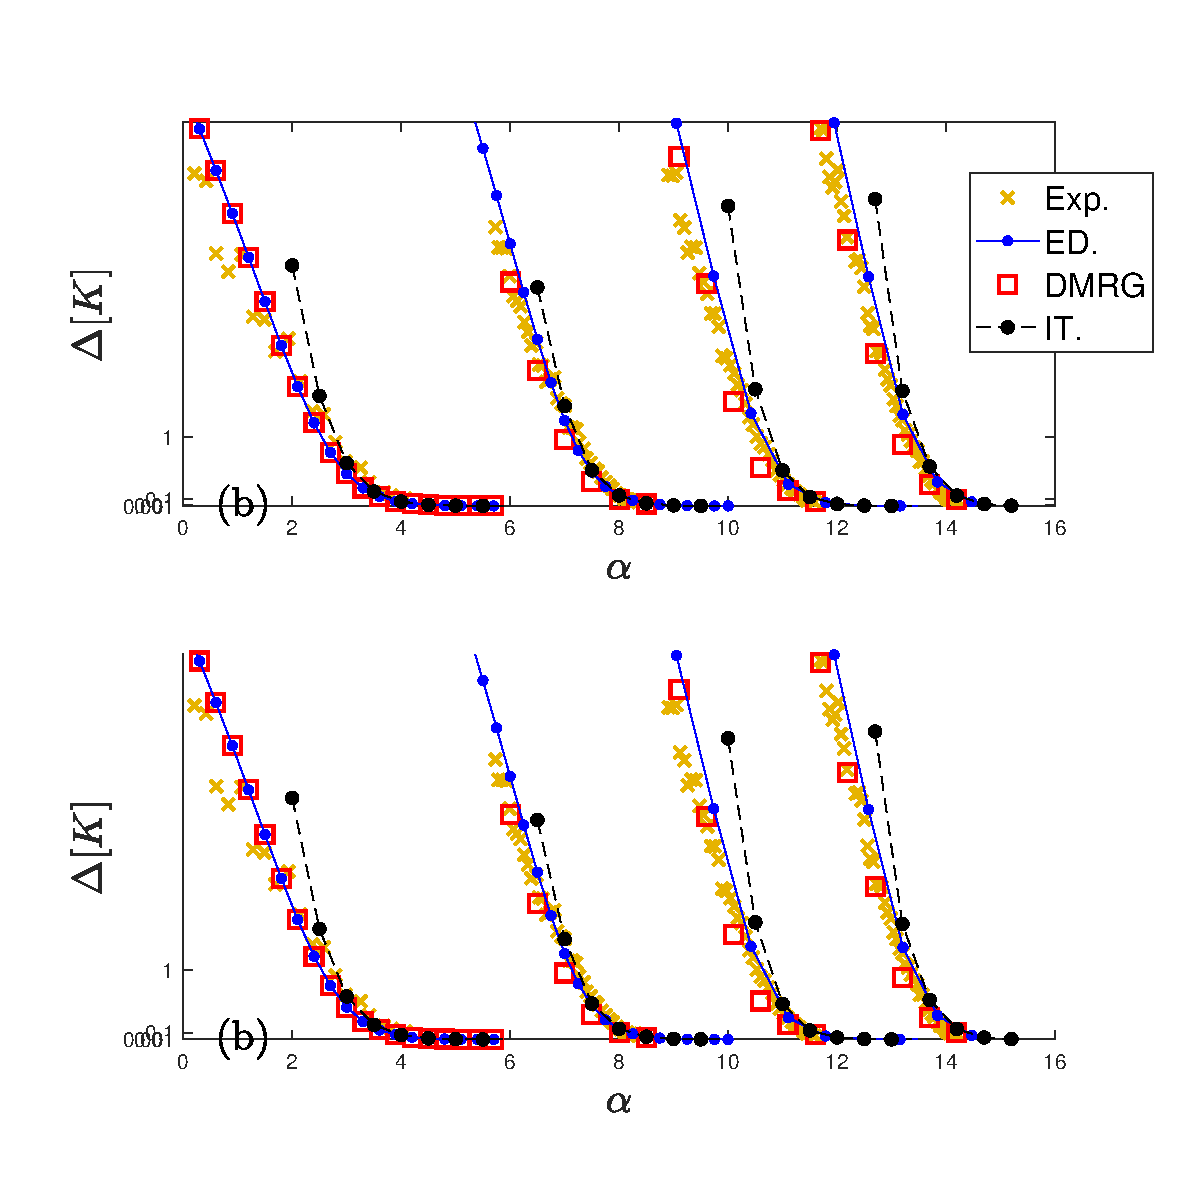
\includegraphics[width=1\columnwidth]{Fig_spectral_gap_exp_fitted_log}&
     		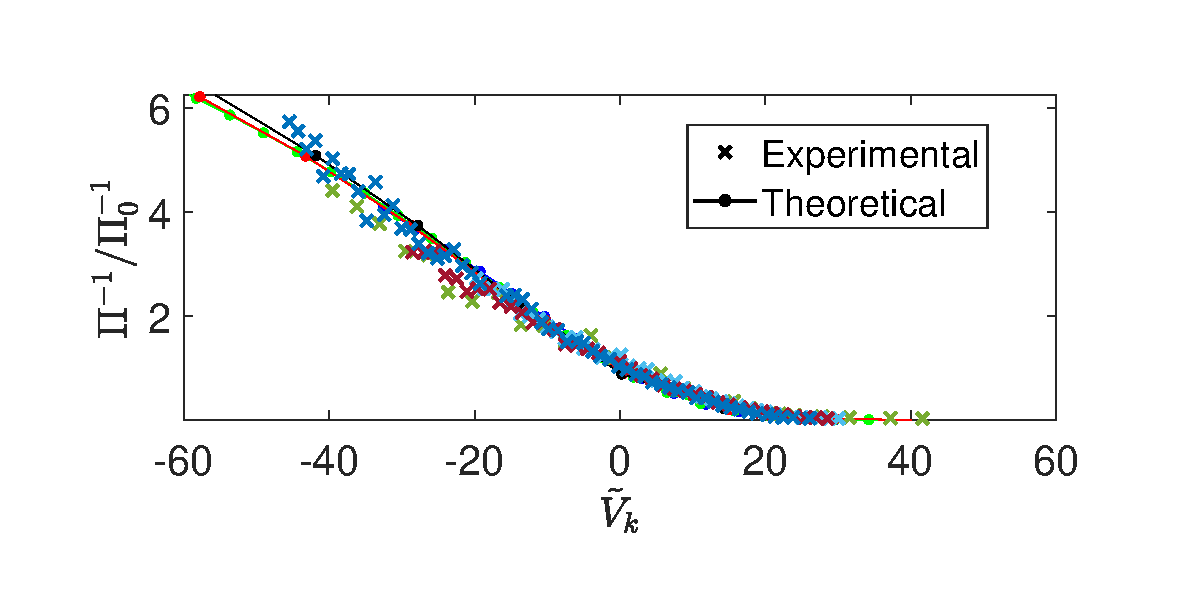
\includegraphics[width=1\columnwidth]{Fig_spectral_gap_exp_log_lin_shahal_scaling_log}
    	\end{tabular}
    	


		 	\caption{(a) and (b) Scaled experimental data for the measured polarization and numerical data for the tunnel splitting suing various approaches as function the confinement parameter $\alpha$ that controls the hight of the barrier between the wells. Different curves correspond to different number of electrons in the system. (c) Perpendicular tunneling renormalization factor $R_0$ calculated from the instanton theory. (d) Demonstraition of the universal scaling between the experimental data and the exact diagonalization calculation. Gate voltage $V_k$ adjusts the potential barrier, and $\Pi_0^{-1}$ is a normalization factor obtained from the experimental curves critical $V_k$ value. (I kept it in it's original form from Shahal's ppt) }
     
     \label{fig:experimental_setup}
    \end{center}
\end{figure*}    
  	

\section{Numerical approaches}
\begin{itemize}
\item Effective Hami
\item alpha values; epsilon values
\item what we calculate, trajectories, tunnel splitting, polarization
\end{itemize}

\begin{equation}
\frac{H}{E_0} = \tilde{H} = \sum_{i = 1}^N \left[ -\frac{1}{2}\frac{\partial^2}{\partial \chi_i^2} - \frac{\alpha}{2}\chi_i^2 + \frac{1}{4} \chi_i^4 \right] + \eta \sum_{i < j}^N \frac{1}{\left| \chi_i - \chi_j  \right|}
\end{equation}

\begin{equation}
l_d = \left( \frac{\hbar^2}{m^* \beta} \right)^{1/6} \approx 160 \,{\rm{ [nm]}}
\end{equation}
\begin{equation}
E_0 = \frac{\hbar^2}{m^* l_d^2} \approx 0.48 \,{\rm{ [meV]}}
\end{equation}

\begin{equation}
\eta = \frac{l_d}{a_B} \approx 20
\end{equation}

\begin{align}
{\text{"Universal scaling"}}\\
\tilde{V}_k &= (V_k - V_{0}^{(n)})f_n \\
\tilde{\Delta} &= \Delta f_y \\
\tilde{\alpha} &= (\alpha - \alpha_0^{(n)}) f_n^{(\alpha)} \\
{\text{Scaling to }} \alpha \\
\alpha &= \alpha_0^{(n)} + \frac{f_n}{f_\alpha^{(n)}} \left(V_k - V_0^{(n)}  \right)
\end{align}
\subsection{DMRG}
\begin{itemize}
\item Basis used
\item I guess technical description here is not that important, myabe in the SUpMat
\end{itemize}

\subsection{ED}
\begin{itemize}
\item general finite difference method description
\item restricted space method
\end{itemize}

\subsection{Instanton}
\begin{itemize}
\item summary of the calculation (details could go to supmat)
\item Zero mode solution
\item Monte Carlo simulation details
\item Validity under a certain alpha
\item Perpendicualr factor
\end{itemize}

     
\section{Tunnel splitting and polarization results}
\begin{itemize}
\item tunnel splitting 
\item Polarization
\item assimptotic matching between results
\end{itemize}

\begin{figure}[h!]
	\begin{center}
		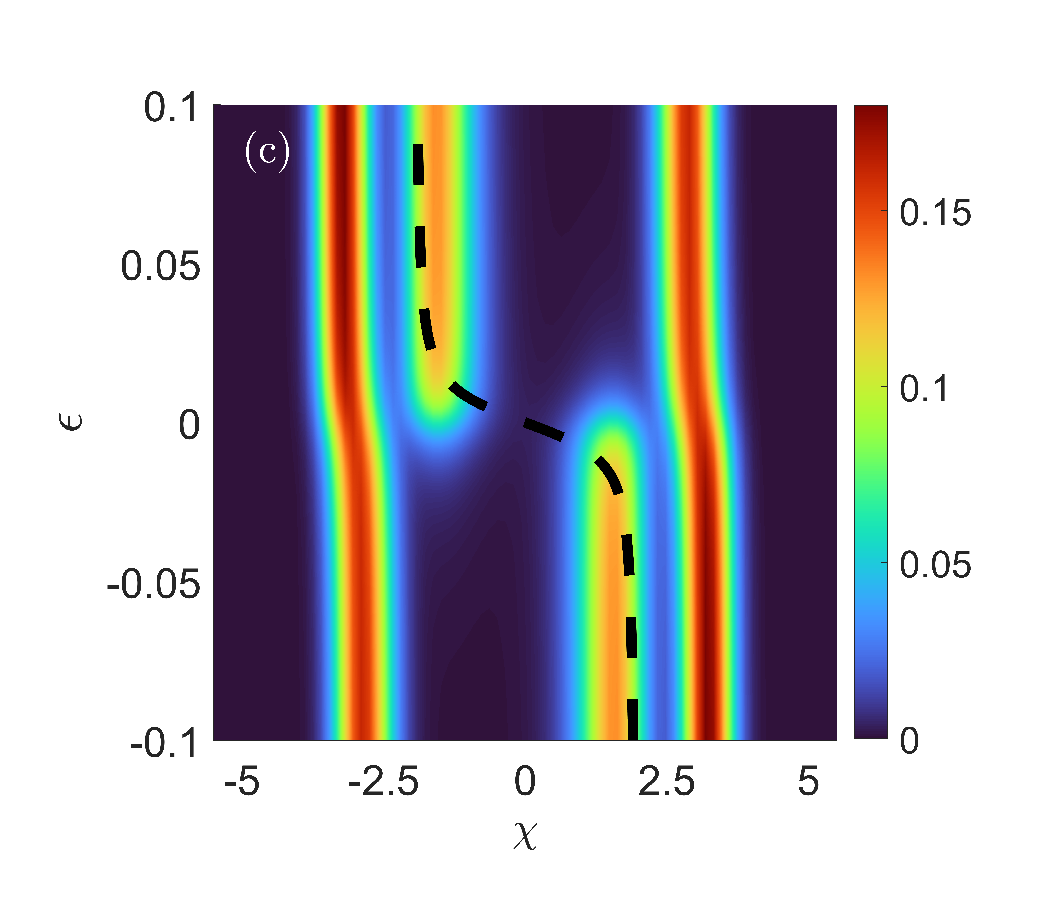
\includegraphics[width=1\columnwidth]{Fig_Polarization_2D}
		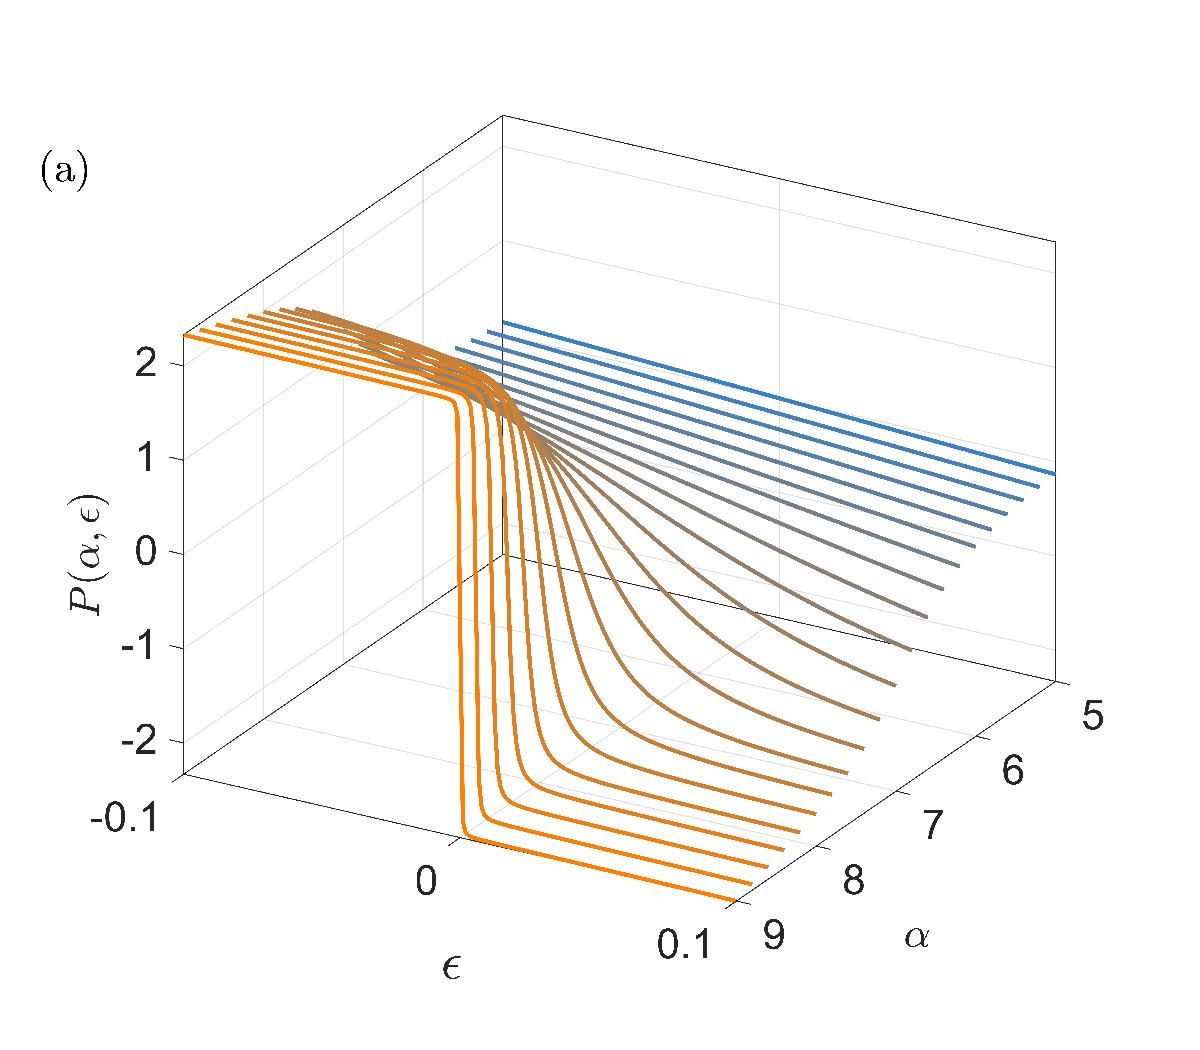
\includegraphics[width=1\columnwidth]{Fig_Polarization_3D_theor}
		\caption{(a) Charge density as a function of the linear detuning parameter $\epsilon$ at $\alpha = 7.8$. The dashed line denotes the polarization in the system. (b) Polarization as a function of $\alpha$ and $\epsilon$.}
	\end{center}
\end{figure}
     

\subsection{Comparison with experiments}
\begin{itemize}
\item Scaling the experiments and the numerical data together
\end{itemize}

	
\section{Conclusion}
\begin{itemize}
\item Quantum fluctuations effects tunneling transition
\item transverse factor renormalize tunneling
\item Scaling with experimental data
\end{itemize}

  

     
 
        
\newpage
\newpage 
\pagebreak
\section{SupMat Figures}


	
	\begin{figure}[h!]
		\begin{center}
			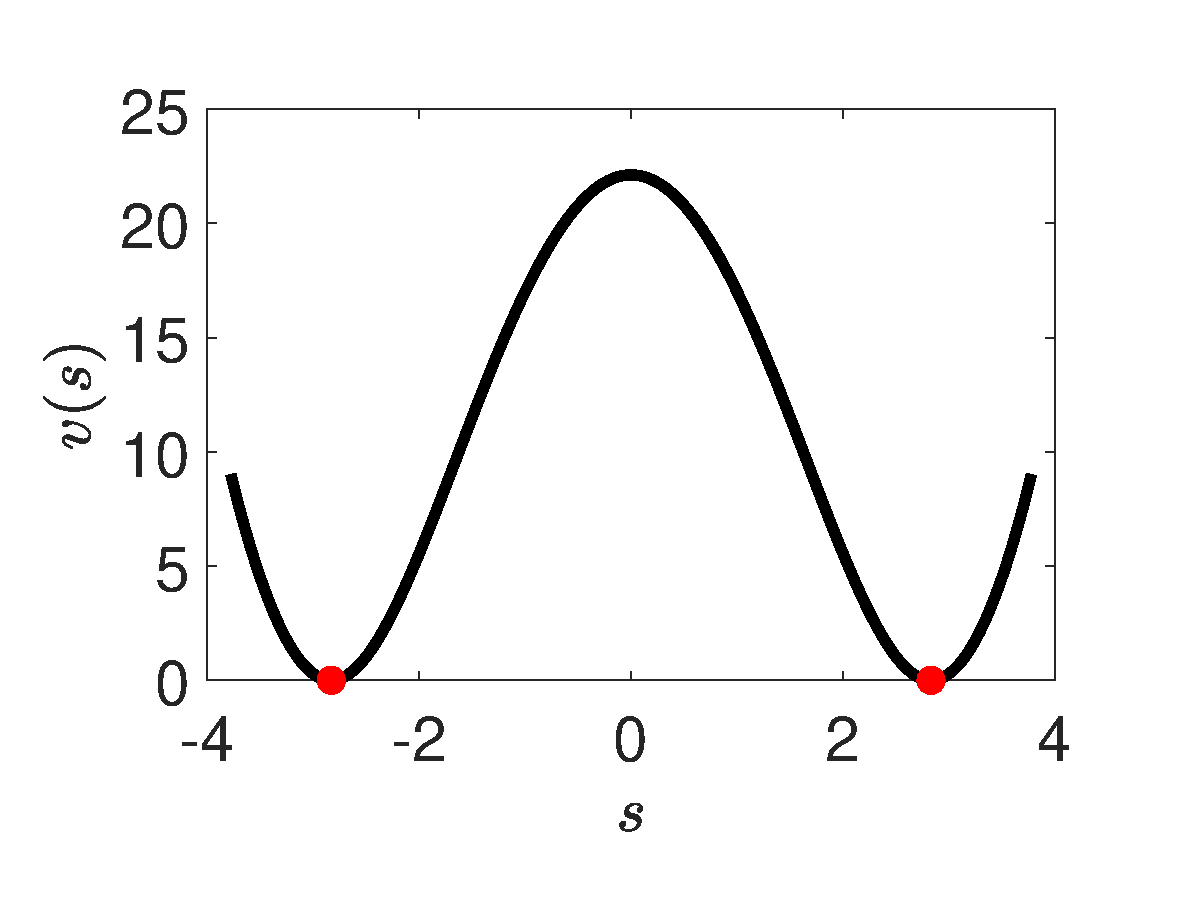
\includegraphics[width=0.9\columnwidth]{SupMatFig_EffectivePotential.pdf}
			
			\caption{  }
			\label{fig:gap}
		\end{center}
	\end{figure}
	
\begin{figure}[h!]
    \begin{center}
     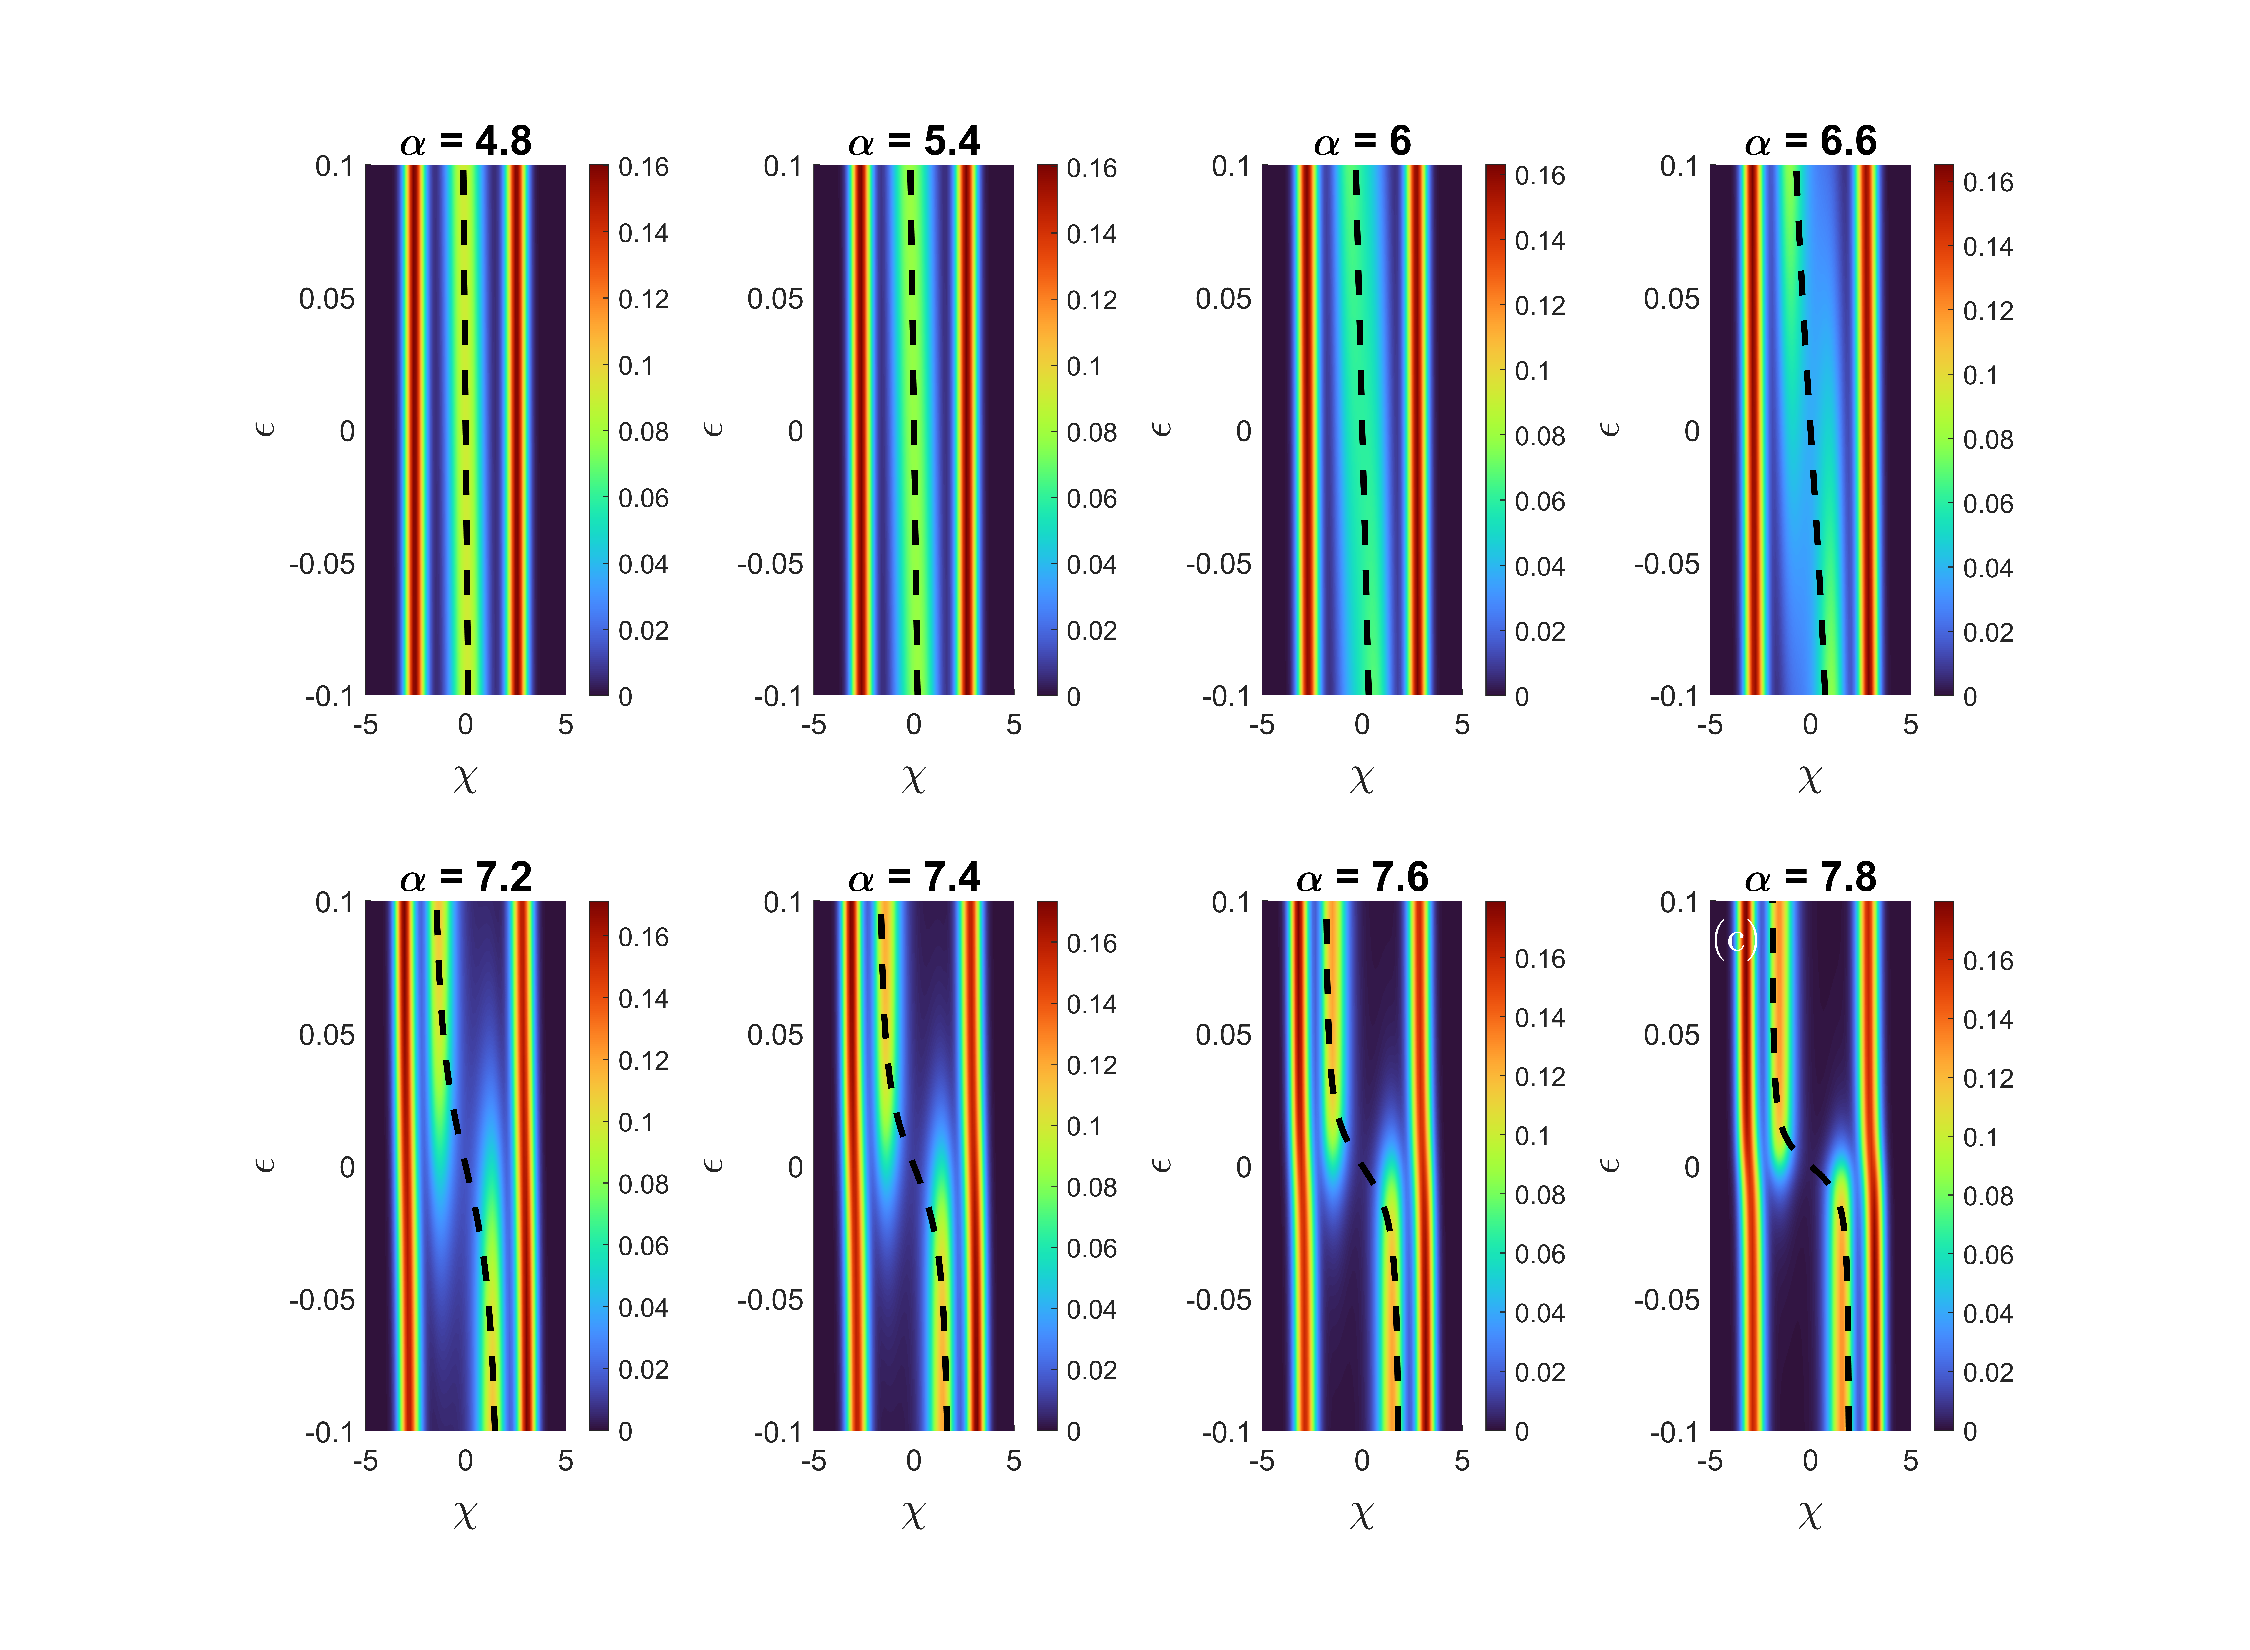
\includegraphics[width=2\columnwidth]{SupMatFig_DensitySeries}
     \caption{caption}
     \label{fig:experimental_setup}
    \end{center}
     \end{figure}

\bibliography{references}
\end{document}
